\subsection{Direct muon (anti)neutrino magnetic moment measurements}
\subsubsection{NOvA (Biao's thesis)}
\begin{itemize}
    \item $\nu_\mu$ only
    \item Only comparing total event counts - 25 events observed and 23.78 expected
    \item Put an upper limit ($90\%$ C.L.) of $\mu_{\nu_\mu}<1.58\times 10^{-9}\mu_B$ with $10.9\%$ systematic uncertainty on the standard model background
    \item Used $3.62\times 10^{20}$ POT of data ($6.74\times 10^{23}$ POT for MC) with $T\theta^2<0.003\textsf{GeV}\times\textsf{Rad}^2$, $0.3<T<0.9\textsf{GeV}$
\end{itemize}

\subsubsection{MiniBooNE}
\begin{itemize}
    \item $\nu_\mu$ only
    \item Observed excess of events (seems a bit too high)
\end{itemize}

\subsubsection{E734 at the Alternating Gradient Synchrotron (AGS) of the Brookhaven National Laboratory}
\begin{itemize}
    \item \textbf{Both $\nu_\mu$ and $\overline{\nu}_\mu$}
    \item $\mu_{\nu_\mu}<8.5\times 10^{-10}\mu_B$
%    \item \href{https://journals.aps.org/prd/abstract/10.1103/PhysRevD.41.3297}
\end{itemize}

\subsubsection{LSND}

\subsection{Direct electron (anti)neutrino magnetic moment measurements}

\subsection{Solar neutrino magnetic moment measurements}
\subsubsection{XENONnT}
First results published in arXiv:2207.11330\cite{XENON:2022mpc} on 22 July 2022.
\begin{itemize}
    \item 5.9 tonne dual-phase liquid xenon TPC dark matter detector
    \item Region Of Interest is (1,140)~keV
    \item Very low background (~5 times lower than XENON1T)
    \item Tritium excluded as the potential background (also in XENON1T)
    \item No excess found - XENON1T excess excluded with ~4$\sigma$
    \item The $90\%$ C.L. upper limit on solar neutrinos with an "enhanced" magnetic moment is \\$\mu_{\nu_{sol}}~<~6.3\times~10^{-12}\mu_B$, the strongest non-astronomical limit so far (see fig.\ref{fig:XENONnTResults})
\end{itemize}

\begin{figure}
    \centering
    \hspace*{1.5cm}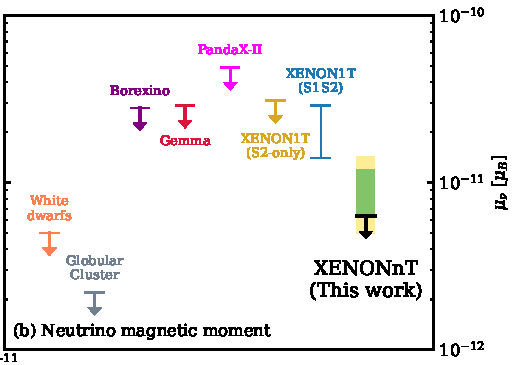
\includegraphics[width=.7\textwidth]{Plots/XENONnTExpResultsComparison.pdf}
    \caption{90\% C.L. upper limit on solar neutrinos with an enhanced magnetic moment.}
    \label{fig:XENONnTResults}
\end{figure}
Amir Khan used\cite{Khan:2022bel} XENONnT's results and derived limits on electromagnetic properties for the three SM neutrino flavours (see fig.\ref{fig:XENONnTFit_Khan}).
\begin{figure}
    \centering
    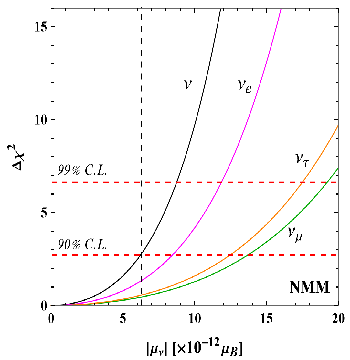
\includegraphics[width=.65\textwidth]{Plots/XENONnTFitForNuMM_Khan.pdf}
    \caption{One-dimensional $\Delta\chi^2$ distribution with 90\% and 99\% C.L. boundaries of neutrino magnetic moments. The distribution in black corresponds to the effective flavor independent magnetic moment}
    \label{fig:XENONnTFit_Khan}
\end{figure}
For $\nu_\mu$ they 

\subsubsection{XENON1T}

\subsubsection{BOREXINO}
Should be $\mu_{\nu_e}<2.8\times 10^{-11}\mu_B$ 
[BorexinoLimit2017.pdf]

\subsubsection{GEMMA}
Should be $\mu_{\nu\ Eff}<2.9\times 10^{-11}\mu_B$. [GemmaLimits2013.pdf] 


\subsection{Other}
\subsubsection{LHC Forward Physics Facilities}
Preliminary sensitivity studies for future experiments (namely for FLArE and FASER$\nu$2)
\begin{itemize}
    \item LHC’s Forward Physics Facilities study high energy (TeV) neutrinos of all flavours from the ATLAS interaction point.
    \item Large opportunity to study tau neutrinos in more detail
\end{itemize}

\subsection{Astrophysics}
[NuMMBasicsAndAstro\_2022.pdf]
Neutrino electromagnetic processes that could be studied/observed in astrophysics
\begin{itemize}
\item Neutrino radiative decay
\begin{itemize}
\item Decay of heavier neutrino flavour into a lighter neutrino and a photon
\item "The neutrino radiative decay has been constrained from the absence of decay photons in studies of the solar, supernova and reactor (anti)neutrino fluxes, as well as of the spectral distortions of the cosmic microwave background radiation."
\item Less stringent than the plasmon decay into a nu-antinu pairs
\end{itemize}
\item Plasmon decay to neutrino-antineutrino pair
\begin{itemize}
\item "For constraining neutrino electromagnetic properties, and obtaining upper bounds on neutrino magnetic moments in particular, the most interesting process is the plasmon decay into a neutrino-antineutrino pair [11]"
\item Plasmon decay frees the energy from the stars plasma in form of neutrinos that escape and therefore speeds up the star cooling
\item "observed properties of globular cluster stars provides new upper bounds on the effective neutrino magnetic moment $\mu_{ef}\leq\left(1.2-2.6\right)\times 10^{-12}\mu_B$ that is valid for both cases of Dirac and Majorana neutrinos."
\end{itemize}
\item Transition of neutrino helicities $\nu_L\rightarrow\nu_R$ from active to sterile neutrinos
\begin{itemize}
\item Supernovas would cool much faster - not observed for 1987A by Kamioka II and IMB, constraining Dirac neutrino mag. moment
\end{itemize}
\end{itemize}
